\chapter{System design}
\label{sec:system_design}
%This chapter will derive the design of the system.
For the system to accomplish the goals stated in \ref{sec:problem}, several hardware and software functions need to be designed and implemented.\\

For the mixed criticality implementation, the hypervisor SafeG~\ref{sec:safeg}~\cite{website:safeg} will be used to alternate between the safety-critical RTOS and the GPOS, as described in section~\ref{sec:lit_emc2mcs}.

\section{Operative system functions}
This section will describe the functions to be implemented on the OS.

\subsection{Longitudinal control}
PID controller
Shared information (safe, control signal)

\subsection{Lane detection}
A lane-detecting algorithm will be implemented on a Raspberry Pi that will send data to the Zedboard/EMC2DP. The choice of Raspberry Pi was made because of the amount of open source video processing code available for the platform. For more info, see the report by Ferhatovic~\cite{ferhatovic2017}.

\subsection{Lateral control}
Lateral control will be implemented on the RTOS on the EMC2DP. The function receives the deviation from the center line as calculated by the lane detection algorithm from the Raspberry Pi, and calculates a control signal from this.

\subsection{Data aggregation}
See the report by~\cite{hellman2017}.

\subsection{Communication}
To establish secure communication between the two vehicles in the platoon, WiFi is used. For more information, see the report by~\cite{lerander2017}.

\section{Hardware implemented functions}
This section will describe the functions to be implemented on the FPGA.

\subsection{Decoder}
To read the speed of the vehicle, encoders are connected to the wheels. The encoders have a resolution of TODO pulses per revolution. The four encoders will send pulses very quickly and a hardware decoder is needed to process them and send the speed of each wheel to the OS.

\subsection{Pulse Width Modulation}
To control the speed of the motor and the position of the steering servo, Pulse Width Modulation (PWM) is used. Two hardware implemented PWM functions will be needed.

\subsection{LIDAR}
To read the distance to the preceding vehicle, a LIDAR (LIght Detection And Ranging) is used. The LIDAR communicates the distance it is reading via a PWM signal. A hardware function is needed to read the PWM pulse and convert it to a distance.

\subsection{Communication}
WiFi communication is used between the two vehicles in the platoon. To read packages, a WiFi module is used that communicates via UART with the EMC2DP. A MicroBlaze in the FPGA processes the packages and sends the parsed data to the OS via a mailbox. For more information, see the report by~\cite{lerander2017}.

\section{Overview design}
An overview of the different functions to be implemented on the Zynq-7000 can be seen in figure~\ref{fig:overview}.

\begin{figure}[H]
\centering
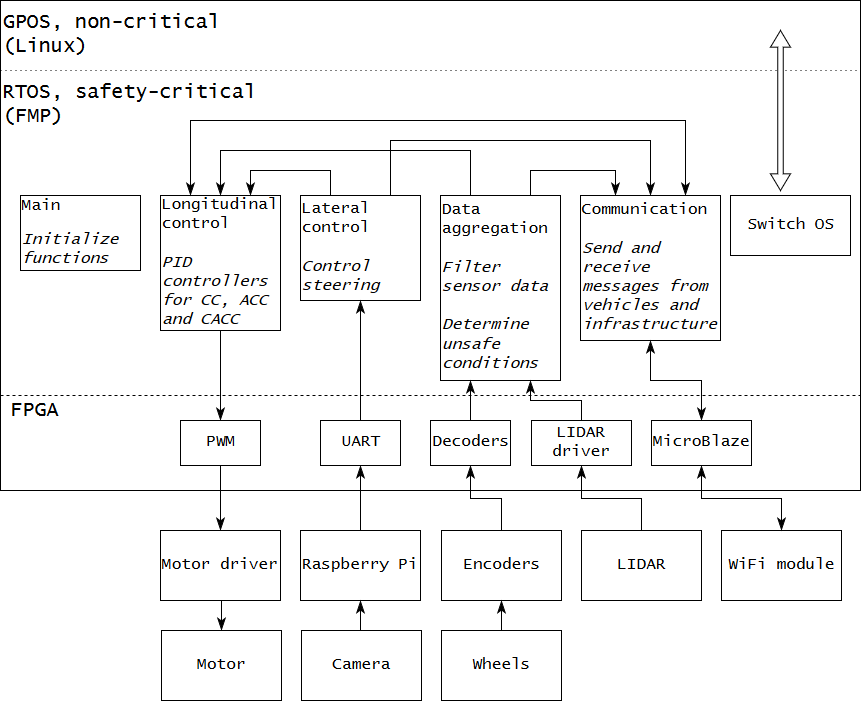
\includegraphics[width=\textwidth]{./img/design_overview.png}
\caption{Overview of the different functions to be implemented.}\label{fig:overview}
\end{figure}

A sequence diagram of the various dependencies and flow of each function can be seen in figure~\ref{fig:sequence}.

\begin{figure}[H]
\centering
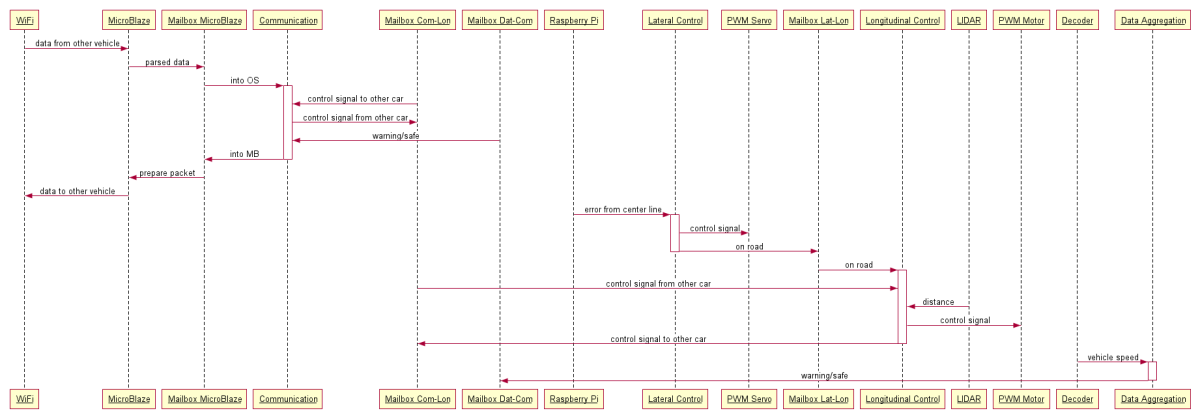
\includegraphics[width=\textwidth]{./img/design_sequence.png}
\caption{Sequence diagram of the various hardware and software functions.}\label{fig:sequence}
\end{figure}

Processor tasks
Dependencies
Flow chart